%
%%%% !BIB TS-program = biber
%%%% !BIB program = biber
% !BIB TS-program = bibtex
% !BIB program = bibtex
% !TeX spellcheck = en_US
% !TeX program = lualatex
%
%
%
% v 2.3  Feb 2019   Volker RW Schaa
%		# changes in the collaboration therefore updated file "jacow-collaboration.tex"
%		# all References with DOIs have their period/full stop before the DOI (after pp. or year)
%		# in the author/affiliation block all ZIP codes in square brackets removed as it was not 
%         understood as optional parameter and ZIP codes had bin put in brackets
%       # References to the current IPAC are changed to "IPAC'19, Melbourne, Australia"
%       # font for "url" style changed to "newtxtt" as it is easier to distinguish "O" and "0"
%
\documentclass[letter,
               %boxit,        % check whether paper is inside correct margins
               %titlepage,    % separate title page
               %refpage       % separate references
               %biblatex,     % biblatex is used
               keeplastbox,   % flushend option: not to un-indent last line in References
               %nospread,     % flushend option: do not fill with whitespace to balance columns
               %hyphens,      % allow \url to hyphenate at "-" (hyphens)
               %xetex,        % use XeLaTeX to process the file
               %luatex,       % use LuaLaTeX to process the file
               ]{jacow}
%
% ONLY FOR \footnote in table/tabular
%
\usepackage{pdfpages,multirow,ragged2e} %
%
% CHANGE SEQUENCE OF GRAPHICS EXTENSION TO BE EMBEDDED
% ----------------------------------------------------
% test for XeTeX where the sequence is by default eps-> pdf, jpg, png, pdf, ...
%    and the JACoW template provides JACpic2v3.eps and JACpic2v3.jpg which
%    might generates errors, therefore PNG and JPG first
%
\makeatletter%
	\ifboolexpr{bool{xetex}}
	 {\renewcommand{\Gin@extensions}{.pdf,%
	                    .png,.jpg,.bmp,.pict,.tif,.psd,.mac,.sga,.tga,.gif,%
	                    .eps,.ps,%
	                    }}{}
\makeatother

% CHECK FOR XeTeX/LuaTeX BEFORE DEFINING AN INPUT ENCODING
% --------------------------------------------------------
%   utf8  is default for XeTeX/LuaTeX
%   utf8  in LaTeX only realises a small portion of codes
%
\ifboolexpr{bool{xetex} or bool{luatex}} % test for XeTeX/LuaTeX
 {}                                      % input encoding is utf8 by default
 {\usepackage[utf8]{inputenc}}           % switch to utf8

\usepackage[USenglish]{babel}

% My packages:
\usepackage{listings}
\usepackage{color}

\definecolor{dkgreen}{rgb}{0,0.6,0}
\definecolor{gray}{rgb}{0.5,0.5,0.5}
\definecolor{mauve}{rgb}{0.58,0,0.82}

\lstset{frame=tb,
  language=Python,
  aboveskip=3mm,
  belowskip=3mm,
  showstringspaces=false,
  columns=flexible,
  basicstyle={\small\ttfamily},
  numbers=none,
  numberstyle=\tiny\color{gray},
  keywordstyle=\color{blue},
  commentstyle=\color{mauve},
  stringstyle=\color{dkgreen},
  breaklines=true,
  breakatwhitespace=true,
  tabsize=3
}

%
% if BibLaTeX is used
%
\ifboolexpr{bool{jacowbiblatex}}%
 {%
  \addbibresource{jacow-test.bib}
  \addbibresource{biblatex-examples.bib}
 }{}
\listfiles

%%
%%   Lengths for the spaces in the title
%%   \setlength\titleblockstartskip{..}  %before title, default 3pt
%%   \setlength\titleblockmiddleskip{..} %between title + author, default 1em
%%   \setlength\titleblockendskip{..}    %afterauthor, default 1em

\begin{document}

\title{WHATRECORD: A PYTHON-BASED EPICS FILE FORMAT TOOL
\thanks{Work supported by U.S. D.O.E. Contract DE-AC02-76SF00515.}}
\author{Kenneth Lauer\thanks{klauer@slac.stanford.edu}, SLAC National Accelerator Laboratory, Menlo Park, CA }
	
\maketitle

%
\begin{abstract}
  \verb_whatrecord_ is a Python-based parsing tool for
  interacting with a variety of EPICS (Experimental Physics and Industrial
  Control System) file formats, including V3 and V7 database files. The project
  aims for compliance with epics-base by using Lark grammars that
  closely reflect the original Lex/Yacc grammars. 

  \verb_whatrecord_ offers a suite of tools for working with its supported file
  formats, with convenient Python-facing dataclass object representations and
  easy JSON (JavaScript Object Notation) serialization. A prototype backend web
  server for hosting IOC (Input/Output Controller) and record information is
  also included as well as a Vue.js-based frontend, an EPICS build system
  \verb_Makefile_ dependency inspector, a static analyzer-of-sorts for startup
  scripts, and a host of other things that the author added at whim to this
  side project.
\end{abstract}

\section{BACKGROUND}

\subsection{The Problem - and the Inspiration}

Before digging into the details of the
\verb_whatrecord_\cite{whatrecord-github}, toolsuite, let us first take a look
at the problem and the inspiration behind its creation.

At the LCLS (SLAC's Linac Coherent Light Source), the accelerator and photon
side control systems include approximately 3000 IOC instances in total, with
hundreds of modules and dozens of versions per module.

In general, these EPICS\cite{epics-base} IOCs, modules, and extensions are
comprised of a conglomeration of unique file formats. Some common examples of
such file formats include:

\begin{Itemize}
  \item Process database files (\verb_.db_)
  \item Database definition files (\verb_.dbd_)
  \item Template / substitutions files
  \item IOC shell scripts (\verb_st.cmd_)
  \item StreamDevice protocols (\verb_.proto_)
  \item State notation language programs (\verb_.st_)
  \item Gateway configuration (\verb_.pvlist_)
  \item Access security files (\verb_.acf_)
  \item Build system \verb_Makefile_s
\end{Itemize}

Additionally, facility-specific tools (centralized IOC management tools like
LCLS's IOC Manager, archiver appliance automation tools, and so on) build on
top of IOCs and records.

Combined, this makes for an enormous code base with a mix of these
EPICS-specific file formats.

Links between these files are often implicit.  Take, for example, that an EPICS
IOC record has a specific record type name alongside its name in a database
file (\verb_.db_), an EPICS PV (Process Variable) name, in a traditional IOC, starts
with the record name defined in a database file. This PV name acts as a global
identifier that allows for clients on the same network subnet to access - and
potentially modify - related data.

A record is made up of fields which can contain metadata like engineering units
or user-specified descriptions, references to other records, relevant data
values, and so on.

An example record instance, defining a single AI (analog input) record named
\verb_IOC:RECORD:NAME_ is as follows:
\begin{lstlisting}[language=bash]
  record(ai, "IOC:RECORD:NAME") {}
\end{lstlisting}

This file does not define what the fields of the record type; that is the
responsibility of the database definition file (.dbd). A simplified excerpt
from a database definition file, defining a single field
for the "ai" record type is as follows:

\begin{lstlisting}[language=bash]
  recordtype(ai) {
      ...
      field(NAME, DBF_STRING) {
          special(SPC_NOMOD)
          size(61)
          prompt("Record Name")
      }
      ...
  }
\end{lstlisting}

Note that there is no explicit link between the database file and the database
definition file: neither reference the other by filename.
Rather, one can only infer the link by examining a third file, the IOC-specific
IOC shell script (.cmd) file, line-by-line.

An excerpt from such a startup script could look like:
\begin{lstlisting}[language=bash]
dbLoadDatabase("path/to/the.dbd",0,0)
IOC_registerRecordDeviceDriver(pdbbase) 
dbLoadRecords("records.db")
\end{lstlisting}

Each line of this script includes up to one command. Each of those commands
has been registered by either EPICS itself, the modules included in the IOC,
or the IOC source code itself.  Typically, the available commands
would be found either in documentation or by executing the IOC and invoking the
built-in help system. Alternatively, the most reliable fallback ends up
being the source code itself.

Other direct or indirect references may be found inside fields.  
For example, depending on the \verb_DTYP_ (device type) field, the \verb_INP_
(input specification) field may be a custom string defined at the device
support layer. Interpretation of this field requires knowledge of how
these are formatted.  Take StreamDevice\cite{streamdevice}, a generic
support module for communicating with controllers that use simple byte
streams for communication, for example:
\begin{lstlisting}[language=bash]
  record(ai, "IOC:RECORD:NAME") {
    field(DTYP, "stream")
    field(INP,  "@ProtocolFilename.proto getValue PS1")
  }
\end{lstlisting}

The device type here is set to \verb_"stream"_, a custom identifier that
StreamDevice has hard-coded.  This instructs EPICS to use StreamDevice
and interpret the \verb_INP_ field with it.  It us up to the IOC developer to
understand the format of these strings and set them appropriately, in order
to reference back to the protocol file that defines the byte string to send
and the expected response format. Here, a StreamDevice protocol file for
the above record indicates that a simple string \verb_WHAT:IS:THE:VALUE?_
is to be sent, and a floating point value (\verb_%f_, as in the C \verb_scanf_
format specifiers) is to be sent from the controller:
\begin{lstlisting}[language=bash]
  getValue {
      out "WHAT:IS:THE:VALUE?";
      in "%f";
  }
\end{lstlisting}

This section is a small but important part of what makes up an IOC: the build
system surrounding all of these files, other modules with their own standards,
access security configuration for intra-subnet access, gateway configuration
controlling inter-subnet access, facility-specific tools that rely on PV
names, and so on further complicate the number of files and references
one needs to be aware of.

While those familiar with EPICS IOC development may find that the above is
obvious and simple, it can be opaque at best to those unable to dedicate the
time to reading through esoteric (and often outdated) manuals or source
code.

\subsection{Goals and the Emergence of whatrecord}

The previous section's problem led the author over the years to desire a tool
that could somehow unify these file formats and provide the ability to inspect
the links.

These initial goals led to the creation of this new Python package,
\verb_whatrecord_:
\begin{itemize}
  \item Allow for easy parsing of all the special formats outside, and
    represent them in a widely-used interchange format like JSON.
  \item Aid the user in the understanding of existing IOCs, whether they are
    deployed and running or not.
  \item Provide a method to see how different records, different IOCs, all
    relate to one another, without requiring the IOC to be running.
  \item Provide a method for cross-referencing a PV name to its database
    file, record definition, startup script, and IOC.
\end{itemize}

With these implemented, pathways for new possibilities were opened: the ability
to linking records to PLC code, to StreamDevice protocol information, to
gateway access rules, and even shell commands to their respective source code.

\section{CORE FUNCTIONALITY}

\subsection{Overview}
\verb_whatrecord_ will parse any of the following into intuitive Python dataclasses
using the Lark\cite{lark} parsing toolkit:
\begin{itemize}
  \item Database files (V3 or V4/V7), database definitions,
    template/substitution files
  \item Access security configuration files
  \item Autosave .sav files
  \item Gateway pvlist configuration files
  \item StreamDevice protocol files
  \item snlseq/sequencer state machine parsing
\end{itemize}

IOC shell scripts (i.e., \verb_st.cmd_) can be interpreted and annotated with
contextual information during the loading process.  The process aims to record
what files were loaded during startup, what records will be available in the
IOC, what errors were found when loading, what file and line did each record
get loaded, and what are the inter- or intra-IOC record relationships.

Additionally, \verb_whatrecord_ offers tools for:
\begin{itemize}
  \item Exporting all parsed results to JSON-serializable objects.
  \item EPICS build system \verb_Makefile_ introspection, a sumo\cite{sumo}-inspired
    implementation.
  \item GDB Python script that inspects binary symbols to find IOC shell
    commands, variables and source code context
    \begin{lstlisting}[language=bash]
  dbLoadRecords [str: fname] [str: subs]
  .../src/ioc/db/dbIocRegister.c:53
    \end{lstlisting}
  \item Accurate EPICS macro handling using epicsmacrolib\cite{epicsmacrolib}.
  \item Linting startup scripts.
  \item Plugins for loading happi devices, TwinCAT PLC projects, and IOC
    information from LCLS’s IOC manager.
  \item Process database record to Beckhoff TwinCAT PLC source code definition
    mapping (when used in conjunction with pytmc\cite{pytmc}).
\end{itemize}

An intuitive Python API, user-facing command-line tools, a web-based
API/backend server to monitor IOC scripts and serve IOC/record information, and
a Vue.js-based frontend single-page application are also provided.

\subsection{Parsing with Lark}

\verb_whatrecord_ utilizes the Lark parser internally to parse most of its supported
file formats.  Lark supports writing custom parsers with EBNF (extended
Backus–Naur form) metasyntax.  It is capable of parsing all context-free
grammars with ambiguity resolution. 

The grammars implemented in \verb_whatrecord_ closely resemble those in EPICS because
the source Lex/Yacc grammars are syntactically similar.  A test suite is
included in \verb_whatrecord_ which attempts to cover various aspects of the packaged
grammars.

Parsing a file in \verb_whatrecord_ results in user-friendly type annotated
\verb_dataclass_ instances. These can be readily inspected programmatically,
serialized to JSON, and - in several cases - exported back into their original
format.

\begin{lstlisting}[language=python]
import whatrecord
db = whatrecord.parse(
    "whatrecord/tests/iocs/db/basic_asyn_motor.db"
)
record = db.records["$(P)$(M)"]
print(record.fields["TWV"].value)  # -> '1'
\end{lstlisting}

A key feature of \verb_whatrecord_'s parsing utilities is that it records the context
of many operations.  When two different files are used to load a record,
both will be present in the context information:

\begin{lstlisting}[language=python]
import whatrecord
ioc = whatrecord.parse(
  "whatrecord/tests/iocs/ioc_a/st.cmd"
)
db = ioc.shell_state.database
record = db["IOC:KFE:A:One"]
print(record.context)
\end{lstlisting}

Yields the following, indicating the files and line numbers used to load the
given database record instance:
\begin{lstlisting}[language=python]
(whatrecord/tests/iocs/ioc_a/st.cmd:13,
 whatrecord/tests/iocs/ioc_a/ioc_a.db:1)
\end{lstlisting}

\subsection{Exporting/Serializing to JSON}

With the \verb_whatrecord_ command-line entry point, you can parse supported formats
and pipe their information to tools like \verb_jq_\cite{jq} to interact and run
basic queries on data.

The following lists all records in a database file and selects a set of
information:
\begin{lstlisting}[language=bash]
  $ whatrecord parse whatrecord/tests/iocs/db/pva/iq.db |
     jq '.records[] | [.name, .record_type, .fields.OUT.value]'
  [
    "$(PREFIX)Rate",
    "ao",
    "$(PREFIX)dly_.ODLY NPP"
  ]
  [
    "$(PREFIX)Delta",
    "ao",
    null
  ]
  ...
\end{lstlisting}

The following inspects some EPICS V4 \verb_Q:Group_ settings:

\begin{lstlisting}[language=bash]
$ whatrecord parse whatrecord/tests/iocs/db/pva/iq.db | 
    jq '.records[] | [ .name, .info["Q:group"]]'
[
  "$(PREFIX)Rate",
  null
]
[
  "$(PREFIX)Phase:I",
  {
    "$(PREFIX)iq": {
      "phas.i": {
        "+type": "plain",
        "+channel": "VAL"
      }
    }
  }
]
...

\end{lstlisting}

\section{FORMATS AND IMPLEMENTATION NOTES}

\subsubsection{Database Files}

\verb_whatrecord_ implements two grammars for EPICS process databases, as there are
significant differences between the grammars used for EPICS V3 and V4+ IOCs.

A flag is available \verb_--v3_ for \verb_whatrecord parse_ to aid facilities
that have not yet opted in to using V4+.

\subsubsection{Access Security Configuration Files (ACF)} whatrecord parses ACF
files that target typical EPICS IOCs along with the EPICS gateway.  This
information can be correlated to records in the frontend, covered in a later
section.

\subsubsection{Substitution Files} Substitutions files and those supported by
\verb_dbLoadTemplate_ are readily supported by \verb_whatrecord_.  Contextual
information as to which files are loaded in the process is reliably carried
along.

A separate grammar for the format used by the command-line tool \verb_MSI_ (the
Macro Substitution and Include tool) is also provided due to their differing
implementations.

\subsubsection{Autosave Save Files} Autosave save files (\verb_.sav_), which
track the state of a record such that it may be restored at the next boot of an
IOC, are supported by \verb_whatrecord_. In the web frontend, these values will
be displayed alongside those in the database file.

\subsubsection{Gateway PV Lists} Gateway \verb_.pvlist_ files are supported by
\verb_whatrecord_.  In the frontend, this allows for the easy correlation of
gateway rules to records that apply to it, and also in reverse, showing which
gateway rules apply to the selected record.

\subsubsection{Sequencer - State Notation Language} The EPICS sequencer's state
notation language format \verb_.st_ files is supported by \verb_whatrecord_
with some caveats. \verb_whatrecord_ does not have full support for a C
preprocessor, which the sequencer relies on.  This means that for simple files
(and those that only use simple C \verb_define_s), \verb_whatrecord_
successfully parses the files, whereas complicated \verb_define_s could fail to
parse with the included grammar.

\subsubsection{LCLS-Specific Formats} At the LCLS, there are additional file
formats that are in common use. The \verb_epicsArch_ format enumerates process
variables that are to be included for recording in its data acquisition system.
\verb_whatrecord_ provides support for this format and allows for linting and
display through the frontend.

The LCLS photon controls team uses the Python suite Bluesky\cite{bluesky} for
slow-speed data acquisition, with approximately 1,000 Ophyd devices indexed in
a happi\cite{happi} database.  \verb_whatrecord_ provides happi integration,
mapping process variables used in Ophyd devices back to their IOCs.

\subsubsection{Startup Scripts} Startup scripts do not have a corresponding
grammar. In the EPICS implementation, the IOC shell parses commands
character-by-character with a custom routine.  \verb_whatrecord_ has a ported
version of this parsing function for maximum compatibility, supporting
redirection and everything else from the original.

\subsubsection{Macro Handling} Files supported by \verb_whatrecord_ often use
the EPICS macro library (macLib) in order to interpolate variables (environment
variables or otherwise) to their corresponding values.

\verb_whatrecord_ uses epicsmacrolib, which is a Cython-wrapped version of
EPICS macLib, under the hood to dutifully reproduce standard EPICS macro
expansion and state tracking.

\subsubsection{Makefiles} \verb_Makefile_s can be inspected to reveal
per-module or per-IOC dependencies and settings of the EPICS build system.
Unlike the other supported formats, \verb_Makefile_s are not parsed but rather
introspected by way of GNU \verb_make_, an optional external requirement.

The implementation is noted as sumo-inspired, as an important part
of how sumo scans source code is replicated. The library executes \verb_make_
with a custom target, enabling the direct handling of any and all
\verb_Makefile_ syntax that the host supports.

\verb_whatrecord_ is able to extract a variety of information from a
\verb_Makefile_ in this manner, exporting information such as the EPICS build
architectures, cross-compiler host architectures, target architectures, the
EPICS base version, configuration paths, release top variables, environment
variable settings, and so on.

\subsection{Backend Server}

Building on top of the parsing tools, \verb_whatrecord_ provides an
aiohttp\cite{aiohttp}-based "backend" server daemon that enables users to query
IOC-related information over a RESTful (REpresentational State Transfer) JSON
interface.

A summary as to how the backend server operates is as follows:

\begin{enumerate}
  \item Find all EPICS IOCs specified by the user (or those listed in LCLS's
    IOC manager tool).
  \item Load the startup scripts with the built-in parsing tools, including
    databases and supported files.
  \item Periodically check previously-loaded files for changes, and re-load
    IOCs.
  \item Listen for clients (or the \verb_whatrecord_ frontend) querying for IOC
    information by way of aiohttp.
\end{enumerate}

\subsection{Command-Line Tools}

\subsubsection{whatrecord Deps} This tool utilizes the \verb_Makefile_ parsing
tools internally to recursively generate a dependency graph of supporting
modules to a given IOC.

\subsubsection{whatrecord Graph} This graphing tool allows for graphing of
records or state notation language transition diagrams. Inter-IOC record links
may be graphed if multiple database files or startup scripts are specified.

\begin{figure}
   \centering
   \includegraphics*[width=.7\columnwidth]{st-simple}
   \caption{A sample state notation language program graph.}
   \label{fig:simple.st}
\end{figure}

\begin{figure}
   \centering
   \includegraphics*[width=.9\columnwidth]{calc-records}
   \caption{A sample record relationship graph.}
   \label{fig:records}
\end{figure}

A sample state notation language graph is shown in Fig.~\ref{fig:simple.st},
and a sample record relationship graph is shown in Fig.~\ref{fig:records}.

\subsubsection{whatrecord Server} This command spawns the backend server.  It
may also be used to export a cached state for offline usage by the frontend.

\subsubsection{whatrecord Lint} This command offers a work-in-progress set of
linting tools, most of which has not yet been well-defined.  The goal for these
tools will be to allow a facility to enforce certain standards for their IOC
files and avoid common pitfalls by detecting issues prior to the IOC boot
process.

\section{WEB FRONTEND}

A Vue.js\cite{vuejs} web-based frontend application is packaged separately in
the \verb_whatrecord_ repository.  It provides a user-friendly view of the information
that \verb_whatrecord_ can parse and aggregate.

A searchable index of records is the primary view.  Record information can be
used to correlate back to other tools and views. For example, when an autosave
configuration is found in an IOC, the frontend will display that information in
a table underneath "Autosave" and annotate the record to show the on-restore
value.

Similarly, StreamDevice protocol files, happi devices, asyn and motor port,
Archiver Appliance, access security groups, and others will be displayed
alongside the record information.  Source code files may be viewed by
clicking on any context link.

Record links, when detected, are displayed as an interactive graph (by way of
\verb_d3-graphviz_\cite{d3graphviz}).  Inter-IOC links can be interactively
investigated in the "PV Map" section.

\begin{figure}
   \centering
   \includegraphics*[width=.9\columnwidth]{whatrecord-asg}
   \caption{whatrecord frontend: a record with access security group settings.}
   \label{fig:whatrecord-asg}
\end{figure}

\begin{figure}
   \centering
   \includegraphics*[width=.9\columnwidth]{whatrecord-ioc-stream-log0}
   \caption{whatrecord frontend: a record with links.}
   \label{fig:whatrecord-links}
\end{figure}

Sample screenshots of the frontend are shown in Figs. \ref{fig:whatrecord-asg}
and \ref{fig:whatrecord-links}.

\subsection{LCLS}
Views for LCLS-Specific tools can be enabled with an environment variable
setting, including a view of happi devices, an LDAP / netconfig settings
viewer, and epicsArch PV listings.

\subsection{GitHub Actions and "Offline" Mode}

A sample repository\cite{gha-sample} is provided to exhibit the "offline" mode
supported by \verb_whatrecord_.

The offline mode utilizes the \verb_whatrecord_ server in continuous
integration to generate a snapshot of the server information. This information
then takes the place of a backend server, requiring only a tarball of JSON in
order to populate the data.

\subsection{Trying whatrecord}

The easiest method to try the frontend alongside the backend is with Docker Compose.

\begin{lstlisting}[language=bash]
$ git clone https://github.com/pcdshub/whatrecord
$ cd whatrecord/docker
$ docker-compose up
\end{lstlisting}
After executing the above, wait for a few minutes and then open
\verb_http://localhost:8896_ in a browser.

The parsing tools can be used directly with a working Python 3.9+ environment:

\begin{lstlisting}[language=bash]
	$ pip install whatrecord
	$ whatrecord --help
\end{lstlisting}

The \verb_whatrecord_ source code is available on
GitHub\cite{whatrecord-github} and documentation is available on GitHub
Pages\cite{whatrecord-docs}.

\ifboolexpr{bool{jacowbiblatex}}%
	{\printbibliography}%
	{%
	% "biblatex" is not used, go the "manual" way
	
	%\begin{thebibliography}{99}   % Use for  10-99  references
	\begin{thebibliography}{99} % Use for 1-9 references
	
	\bibitem{whatrecord-github}
    	whatrecord: source code repository,\\
		\url{http://www.github.com/pcdshub/whatrecord}
	
	\bibitem{epics-base}
		EPICS,
		\url{http://www.aps.anl.gov/epics/}
	
	\bibitem{streamdevice}
		StreamDevice support,\\
		\url{https://paulscherrerinstitute.github.io/StreamDevice/index.html}
	
	\bibitem{lark}
		Lark: a parsing toolkit for Python,\\
		\url{https://github.com/lark-parser/lark/}
	
	\bibitem{sumo}
		sumo: EPICS support module manager,\\
		\url{https://epics-sumo.sourceforge.io/}
	
	\bibitem{epicsmacrolib}
    	epicsmacrolib: EPICS-compliant macro handling,\\
		\url{https://github.com/pcdshub/epicsmacrolib}
	
	\bibitem{pytmc}
   		pytmc: TwinCAT PLC Code to EPICS Database Tool,\\
		\url{https://github.com/pcdshub/pytmc/}

	\bibitem{jq}
		jq: JSON filter command-line tool,\\
		\url{https://jqlang.github.io/jq/manual/}
	
	\bibitem{bluesky}
    Bluesky,
		\url{https://blueskyproject.io/}
	
  \bibitem{happi}
    happi: the LCLS ophyd device database,\\
    \url{https://github.com/pcdshub/happi/}

	\bibitem{aiohttp}
		aiohttp: an asyncio HTTP client/server,\\
		\url{https://docs.aiohttp.org/en/stable/}
	
	\bibitem{vuejs}
    Vue.js,
		\url{https://vuejs.org/}
	
	\bibitem{d3graphviz}
    d3-graphviz,\\
		\url{https://github.com/magjac/d3-graphviz}
	
	\bibitem{gha-sample}
		GitHub Actions and whatrecord sample,
		\url{https://github.com/pcdshub/ioc-whatrecord-example}
	
	\bibitem{whatrecord-docs}
    	whatrecord: documentation,\\
		\url{http://pcdshub.github.io/whatrecord}
	
	\end{thebibliography}
} % end \ifboolexpr

%
% for use as JACoW template the inclusion of the ANNEX parts have been commented out
% to generate the complete documentation please remove the "%" of the next two commands
% 
%%%%\newpage

%%%%%
% !TeX spellcheck = en_US
%
\twocolumn[\vspace*{-1.8ex}\section{ANNEX A:\endgraf FORMATTING OF AUTHORS AND AFFILIATIONS}\vspace*{\baselineskip}]

\flushcolsend

The names of authors, their organizations/affiliations
and postal addresses should be grouped by affiliation and
listed in \SI{12}{pt} upper- and lowercase letters. The name of
the submitting or primary author should be first, followed
by the coauthors, alphabetically by affiliation. If the
author list for a given affiliation spans multiple lines,
please be sure to break the line in a manner that does not
split the author’s initials from the author’s last name. This
is easily done by placing unbreakable spaces between the
initials and last name. The affiliation name and address
are also best kept together on the same (but not necessarily
separate) line, wherever possible. (See, for example,
the entry for GSI in the following). In cases where authors
have multiple affiliations, the secondary affiliation is
inserted below the author/primary affiliation listing and is
indicated with a superscript, as shown in the following.


Footnotes on the title and author lines may be used for
acknowledgments and e-mail addresses, using a non-numeric
sequence of characters (\textsuperscript{*}, \textsuperscript{†},
\textsuperscript{‡}, \textsuperscript{§}, \textsuperscript{\P}
as generated by \LaTeX's \verb|\footnote| command).

For examples of the preferred formatting of authors and
affiliations, please consult the following list of JACoW
collaboration members.

For manuscripts submitted by large collaborations with
potentially many tens of authors and where, additionally,
there may be page number limitations, a format consisting
of the principle author’s name and institute, followed by
“on behalf of the \ldots\ collaboration”, is preferred.


\clearpage
%
% Include the title/author page of the JACoW Coolaboration
%
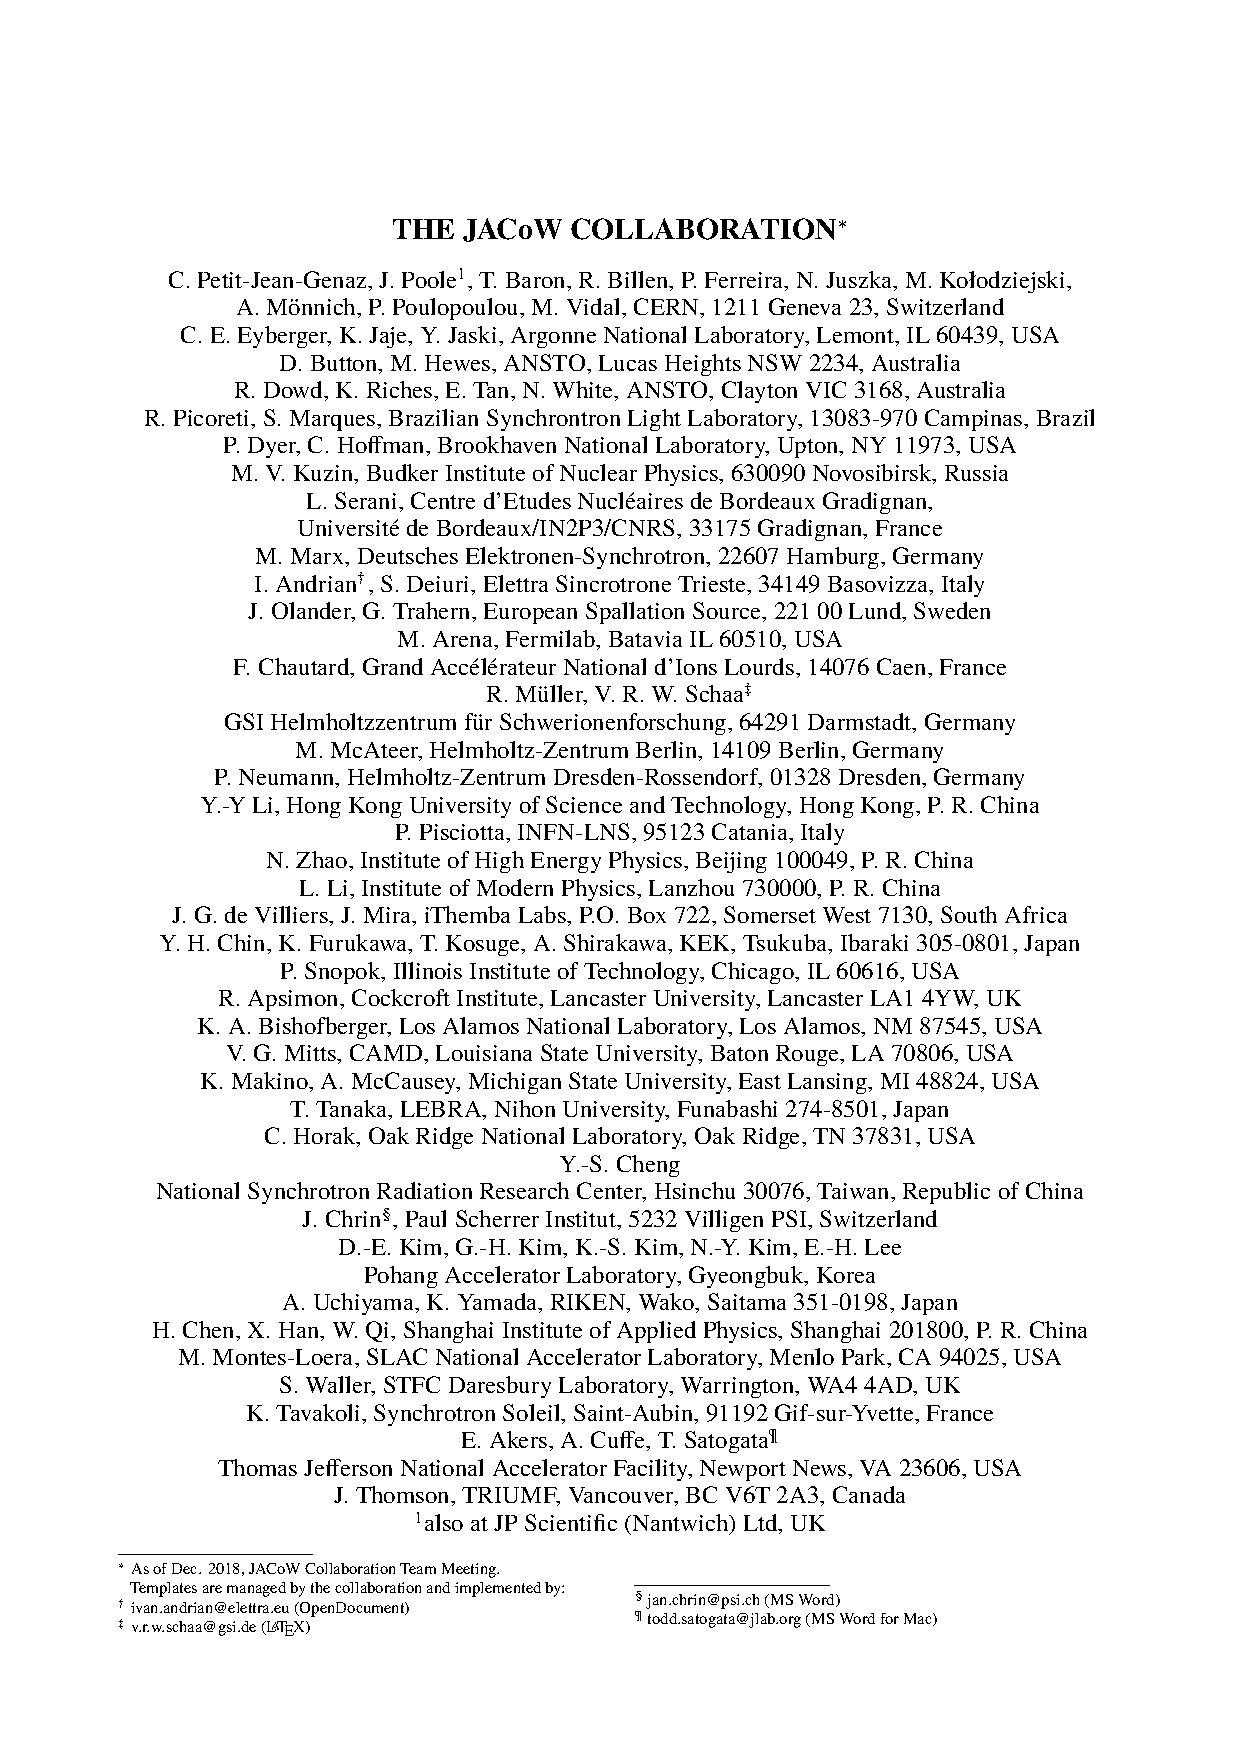
\includepdf[pages=-, noautoscale, pagecommand={}]{jacow-collaboration.pdf}{}

\clearpage

\twocolumn[\vspace*{-1.8ex}\section{ANNEX B:\endgraf IEEE REFERENCE STYLE GUIDE AS APPLIED TO \NoCaseChange{JACoW} PAPERS, \break PERIODICALS AND OTHER WORKS}\vspace*{\baselineskip}]

\subsection{Referencing JACoW Proceedings}

The format for published JACoW proceedings papers is detailed in the following 
and can also be readily deduced from Refs.~[1-3]. At the very minimum, sufficient 
information should be given to enable readers to clearly identify the paper and 
to facilitate its import into digital databases.
\vspace*{-.6\baselineskip}

\subsubsection{Author Listing} Careful attention should be given to the
placing of commas and the use of ‘and’ in the author list.
In particular, for the case of three or more authors
(as in [3]), a comma also follows the penultimate author.
The preference for ‘\emph{et al.}’\ takes precedence when the number
of authors becomes large (e.g., $>$6).
\vspace*{-.6\baselineskip}

\subsubsection{Paper Title} As is modern practice in references, the title
of the paper is written in sentence case, i.\,e., only the
initial letter of the first word in the title is capitalized.
Proper nouns, however, also have a capital. Capital letters
appearing in acronyms likewise remain unaltered
\vspace*{-.6\baselineskip}

\subsubsection{Conference Proceedings} The title of the proceedings is
written in title case in italics using standard abbreviations,
such as \emph{Int.} and \emph{Conf.} The preposition, ``in'', in normal
font, precedes the proceedings title. The location,
i.\,e., city, state (if USA), and country of the conference
venue, the month (three-letter abbreviation) and the year
the conference took place, is then listed. Finally, details
pertaining to the paper itself, such as the conference paper
ID, mandatory page numbers, and the digital object
identifier (DOI), if existing, are listed in the given order.
A monospaced font for the DOI is used so as to help
distinguish it from normal text. In \LaTeX{}
the ‘url’ package is used. The Word template uses the Liberation
Mono TrueType font (size 8 pt), or Lucida Sans Typewriter
font (size 7.5 pt) in earlier Word versions where the Liberation
Mono font may not be available. In LaTeX, the ‘url’
package is used with its default font now being switched to 
``newtxtt'' which offers a better distinction between 
``\texttt{O}'' and ``\texttt{0}''. The conference
paper ID is optional and may be included in the absence
of a DOI to facilitate a search through internet search
engines. DOIs have been assigned to all JACoW
publications appearing in recent proceedings and will
likewise be assigned to articles from conferences further
past, in due course. The use of DOIs is strongly
emphasized.

The complete or abbreviated form for citations, as
shown in the following section, is advocated. The former
is more informative to readers outside the immediate
conference sphere, and will further serve to avoid
potential ambiguities in cases where an acronym is not
unique. Both forms, however, when adhered to, ensure a
proper import into digital libraries and information
sources such as INSPIRE, Scopus, and Google Scholar.
Authors are also reminded to make a distinction between
papers published in JACoW proceedings (which have
page numbers and, in the case of recent publications,
DOIs) and those papers that may have been presented at
past JACoW conferences but were not published~[4].
References to contributions presented at the same
conference should be written as shown in [5]; the wording
“this conference” may be optionally appended.

\subsection{Referencing Periodicals and Other Sources}

The IEEE style is also shown for periodicals [6-11],
online sources [12], books [13, 14], internal reports [15],
theses [16], manuals or handbooks [17], patents [18] and
unpublished material [19, 20]. When citing a periodical,
only the official abbreviation of the journal should be used
[21]. Examples of correctly formatted references can also be 
found at the JACoW website, under ‘Formatting Citations’ which 
is reached through the ‘for Authors’ link.

\subsection{Alignment of References}

In the \LaTeX{} template, \verb|\bibliography{9}| is used for
when the total number of references is less than ten. This
should be changed to \verb|\bibliography{99}| if the number of
references is ten or more.

\patchcmd\thebibliography{\section*{REFERENCES\@mkboth {REFERENCES}{REFERENCES}}}{}{}{}
\section{PAPER PUBLISHED IN A CONFERENCE PROCEEDINGS}

\definecolor{jgreen}{cmyk}{0.81, 0.00, 0.97, 0.00}
\definecolor{jred}{cmyk}  {0.00, 0.99, 1.00, 0.00}
\definecolor{jgrepc}{cmyk}{0.74, 0.05, 1.00, 0.00}
\definecolor{jblue}{cmyk} {0.87, 0.54, 0.00, 0.00}
\definecolor{jvio}{cmyk}  {0.41, 0.82, 0.00, 0.00}
\definecolor{jbook}{cmyk} {0.28, 0.88, 0.79, 0.25}
\definecolor{jrept}{cmyk} {0.07, 0.70, 1.00, 0.00}
\definecolor{jmanu}{cmyk} {0.28, 0.77, 1.00, 0.23}
\definecolor{junpu}{cmyk} {0.00, 0.83, 0.65, 0.00}


\subsection{Complete Form}

\newcommand{\CCom}[2]{\newline\textcolor{#1}{[#2]}}
%\begin{thebibliography}{99}   % Use for  10-99  references
\begin{thebibliography}{9} % Use for 1-9 references
	
	\bibitem{item:1-1}
	A.~Alpha and B.~T.~Beta, “Novel techniques for future TeV electron accelerators,”
	in \textit{Proc.\ 9th Int.\ Particle Accelerator Conf.\ (IPAC’18)},
	Vancouver, BC, Canada, Apr.-May 2018.
	pp. 567-569. \url{doi:10.18429/JACoW-IPAC2017-PAPERID}
	\CCom{jgreen}{Conference Proceedings, two authors; DOI encouraged}

	\bibitem{item:1-2}
	A.~Alpha \emph{et al.},
	“A novel injector,” in \emph{Proc.\ 29th Linear Accelerator Conf.\ (LINAC’18)},
	Shanghai, China, Sep.\ 2018, pp.\ 27-31. %\newline
	\url{doi:10.18429/JACoW-LINAC2018-PAPERID}
	\CCom{jgreen}{Conference Proceedings, for six or more authors use \emph{et al.};	
		 DOI encouraged}
	
	\bibitem{item:1-3}	
	A.~Alpha, B.~T.~Beta, C.~Gamma, and D.~Delta,
	“An overview of control systems,”
	in \emph{Proc.\ 13th Int.\ Conf.\ on Accelerator and Large Experimental Physics Control Systems (ICALEPCS’11)}, Grenoble, France, Oct.\ 2011,
	paper TUP014, pp.\ 89--91.
	\CCom{jgreen}{Conference Proceedings, four authors; optional paper ID
	in the absence of a DOI}
\end{thebibliography}

\vspace*{-.5\baselineskip}
\subsection{Abbreviated Form}

\begin{thebibliography}{9} % Use for 1-9 references
	\bibitem{item:2-1}
	A.~Alpha and B.~T.~Beta, “Novel techniques for future TeV electron accelerators,”
	in \textit{Proc.\ IPAC’18}, Vancouver, BC, Canada, Apr.-May 2018,
	pp.\ 567-569. %\newline
	\url{doi:10.18429/JACoW-IPAC2018-PAPERID}
	\CCom{jgreen}{Conference Proceedings, two authors; DOI encouraged}
	
	\bibitem{item:2-2}
	A.~Alpha \emph{et al.},
	“A novel injector,” in \emph{Proc.\ LINAC’18},
	Shanghai, China, Sep.\ 2018, pp.\ 27-31. %\newline
	\url{doi:10.18429/JACoW-LINAC2018-PAPERID}
	\CCom{jgreen}{Conference Proceedings, for six or more authors use \emph{et al.}; DOI encouraged}
	
	\bibitem{item:2-3}	
	A.~Alpha, B.~T.~Beta, C.~Gamma, and D.~Delta,
	“An overview of control systems,”
	in \emph{Proc.\ ICALEPCS’11}, Grenoble, France, Oct.\ 2011,
	paper TUP014, pp.\ 89--91.
	\CCom{jgreen}{Conference Proceedings, four authors; optional paper ID
				  in the absence of a DOI}
\end{thebibliography}

\section{UNPUBLISHED PAPER PRESENTED AT A PREVIOUS CONFERENCE}


\subsection{Complete Form}

\begin{thebibliography}{9} % Use for 1-9 references
\setcounter{enumi}{3}
 \bibitem{item:41}
	A.~Alpha and B.~T.~Beta,
	“An interesting talk but paper not submitted,”
	presented at the 5th Int.\ Particle Accelerator Conf.\ (IPAC’14),
	Dresden, Germany, Jun.\ 2014, paper MOAX01, unpublished.
	\CCom{jred}{Unpublished paper; conference name in normal font; paper
	ID may only be given if material supplementing the proceedings
	exists on the JACoW website, e.\,g., PDF of talk}
\end{thebibliography}

\subsection{Abbreviated Form}

\begin{thebibliography}{9} % Use for 1-9 references
\setcounter{enumi}{3}
 \bibitem{item:42}
	A.~Alpha and B.~T.~Beta,
	“An interesting talk but paper not submitted,”
	presented at IPAC’14,
	Dresden, Germany, Jun.\ 2014, paper MOAX01, unpublished.
	\CCom{jred}{Unpublished paper; conference name in normal font; paper
	ID may only be given if material supplementing the proceedings
	exists on the JACoW website, e.\,g., PDF of talk}
\end{thebibliography}


\section{PAPER PRESENTED AT THE CURRENT CONFERENCE}

\subsection{Complete Form}

\begin{thebibliography}{9} % Use for 1-9 references
\setcounter{enumi}{4}
 \bibitem{item:51}
	A.~Alpha and B.~T.~Beta,
	“An interesting talk at this conference,”
	presented at the 10th Int.\ Particle Accelerator
	Conf.\ (IPAC’19), Melbourne, Australia, May 2019, 
	paper MOAB01, this conference.
	\CCom{jgrepc}{Current conference; conference name in normal font; 
				  the wording “this conference” is optional}
\end{thebibliography}

\subsection{Abbreviated Form}

\begin{thebibliography}{9} % Use for 1-9 references
\setcounter{enumi}{4}
	\bibitem{item:52}
	“An interesting talk at this conference,”
	presented at IPAC’19, Melbourne, Australia, May 2019, 
	paper MOAB01, this conference.
	\CCom{jgrepc}{Current conference; conference name in normal font; 
				  the wording “this conference” is optional}
\end{thebibliography}


\vspace*{-.5\baselineskip}
\section{PAPER PUBLISHED IN, OR SUBMITTED TO, A PERIODICAL}

\begin{thebibliography}{99} % Use for 1-9 references
  \setcounter{enumi}{5}
	\bibitem{item:6}
		P.~Mercury \emph{et al.},
		“Title of paper published in journal,”
		\emph{Phy.\ Rev.\ Lett.}, vol.\ 114, no.\ 5,
		p.\ 050511, Feb.\ 2014.
		\url{doi:10.1103/PhysRevLett.114.050511}
	\CCom{jblue}{Periodical, Phys.\ Rev.\ Lett.;
		             issue no.\ and month may be omitted}

	\bibitem{item:7}
		P.~Venus \emph{et al.},
		“New techniques in laser wakefield accelerators,”
		\emph{Phys.\ Rev.\ ST Accel.\ Beams}, vol.\ 18,
		p.\ 120198, Dec.~2015. %\newline
		\url{doi:10.1103/PhysRevAccelBeams.18.120198} 
	\CCom{jblue}{Periodical, Phys.\ Rev.\ ST Accel.\ Beams;
			              month may be omitted}

	\bibitem{item:8}
		T.~Earth \emph{et al.},
		“Low dose irradiation impact on modern silicon detectors,”
		\emph{Nucl.\ Instr.\ Meth.}, vol.\ 692, pp.\ 256--280, 2014.
		\url{doi:10.1016/j.nima.2014.11.022}
	\CCom{jblue}{Periodical, Nucl. Instr. Method.}
	
	\bibitem{item:9}
		T.~Earth, L.~Moon, and A.~Belt,
		“Temporal correlations of x-ray free electron lasers,”
		\emph{Optics Express}, vol.\ 20, pp.\ 11396--11404, 2012.
		\url{doi:10.1364/OE.20.11396}
	\CCom{jblue}{Periodical, Optics Express}

	\bibitem{item:10}
		J.~B.~Good,
		“A paper accepted for publication,”
		\emph{Phys.\ Rev.\ Lett.}, to be published.
	\CCom{jblue}{Periodical, paper accepted for publication
		              by Phys. Rev. Lett.}

	\bibitem{item:11}
		G.~D.~Read,
		“Title of paper submitted for publication,”
		submitted for publication.
	\CCom{jblue}{Paper submitted for publication; the name of the
					  periodical does not appear}
\end{thebibliography}

\vspace*{-.5\baselineskip}
\section{ONLINE SOURCE}

\begin{thebibliography}{99} % Use for 1-9 references
  \setcounter{enumi}{11}
	\bibitem{item:121}
		JACoW, \url{http://www.jacow.org} 
		\CCom{jvio}{online source; no hyperlink, no period at end of URL unless there is a trailing “/” as shown below. A monospaced font should be used, this is achieved using the ‘url’ package in \LaTeX}

  \setcounter{enumi}{11}
	\bibitem{item:122}
		JACoW, \url{http://www.jacow.org/}.  
		\CCom{jvio}{online source; no hyperlink, period after trailing “/” in URL
					if optionally preferred. A monospaced font should be used, this is
					achieved using the ‘url’ package in \LaTeX}

\end{thebibliography}

\section{CITATIONS TO BOOKS}

\begin{thebibliography}{99} % Use for 1-9 references
	\setcounter{enumi}{12}
	\bibitem{item:13}
		T.~Earth and L.~Moon,
		“Title of chapter in the book,”
		in \emph{Title of Book}, R Mars, Ed.\ New York, NY, USA:
		Wiley, 1994, pp.\ 42--48. 
	\CCom{jbook}{Chapter in book}
	
	\bibitem{item:14}
		A.~Belt, \emph{Title of Book}. Cambridge, MA, USA:
		MIT Press, 1986. 
	\CCom{jbook}{Book}
\end{thebibliography}

\section{REPORTS AND THESES}

\begin{thebibliography}{99} % Use for 1-9 references
	\setcounter{enumi}{14}
	\bibitem{item:15}
		G. Jupiter \emph{et al.},
		“Title of report,” CERN, Geneva, Switzerland,
		Rep.\ CERN-2012-333, Oct.\ 2012.
	\CCom{jrept}{Report}

	\bibitem{item:16}
		A.~Student, “Title of thesis,”
		Ph.D.\ thesis, Phys.\ Dept.,
		Karlsruher Institut für Technologie, Karlsruhe,
		Germany, 2014.
	\CCom{jrept}{Thesis}
\end{thebibliography}

\section{MANUAL}

\begin{thebibliography}{99} % Use for 1-9 references
	\setcounter{enumi}{16}
	\bibitem{item:17}
		\emph{IEEE Editorial Style Manual},
		IEEE Periodicals,
		Piscataway, NJ, USA, Oct.\ 2014, pp.\ 34-52;
		\url{http://www.ieee.org/documents/style_manual.pdf} 
	\CCom{jmanu}{Handbook/Manual, no hyperlink, no period after URL}
\end{thebibliography}

\section{PATENTS}

\begin{thebibliography}{99} % Use for 1-9 references
	\setcounter{enumi}{17}
		\bibitem{item:18}
		A.~N.~Inventor,
		“Title of patent,”
		Patent Authority and No., Jan.\ 20, 2016.

\end{thebibliography}

\section{UNPUBLISHED WORK AND PRIVATE COMMUNICATION}

\begin{thebibliography}{99} % Use for 1-9 references
	\setcounter{enumi}{18}
	\bibitem{item:19}
		P.~Neptune, “Title of paper,” unpublished.
	\CCom{junpu}{Unpublished}
	
	\bibitem{item:20}
	P.~Uranus, private communication, Jun.\ 2015.
	\CCom{junpu}{Private communication}
\end{thebibliography}

\newpage

\section{JOURNAL ABBREVIATIONS}

\begin{thebibliography}{99} % Use for 1-9 references
	\setcounter{enumi}{20}
	\bibitem{item:21}
		\url{https://woodward.library.ubc.ca/researchhelp/journal-abbreviations/}

\end{thebibliography}

\newpage

\twocolumn[\vspace*{-1.8ex}\section{ANNEX C:\endgraf THE DILIGENT AUTHOR’S CHECKLIST}\vspace*{\baselineskip}]
\flushcolsend

\subsection{Common Oversights}

In order to lessen the load on a small team of editors
and to help expedite publication of the Proceedings, authors
are kindly asked to give themselves an extra few
minutes to go over the following points, which highlight
the most common errors, before uploading their paper. By
providing a properly formatted JACoW paper, the Proceedings
Office is able to benefit from an autodistill process
which automatically converts the author's PDF file
into a version that adheres to the JACoW-compliant PDF
standard. The process further ensures that all fonts required
to view the entire document are embedded, rendering
a final PDF that qualifies technically for publication.


\subsection{Author and Affiliation Listing}

The names of authors and their affiliations should be in
\SI{12}{pt} uppercase and lowercase letters, with standard,
roman fonts (i.\,e., not italics). When there is more than
one author, the submitting author should be first, followed
by the coauthor. Coauthors should be grouped by affiliation
and then be listed alphabetically. Please refer to \textbf{ANNEX~A}
for further details and examples, particularly for
the case where authors have multiple institutes.

\subsection{SPMS Database and Final Manuscript Validation}

Primary authors are reminded that it is their
responsibility to verify the accuracy of the title, abstract,
and coauthor/institute listing, and that these are identical
in both the final manuscript and SPMS database. This is
required to ensure the proper indexing of author/coauthor(s) 
appear in the published proceedings.

\subsection{Subsection Headings}

Subsection Headings are in \SI{12}{pt} \emph{italic} lowercase and uppercase.
The initial letter of every principle word is capitalized,
and the heading is left aligned in the column.

\subsection{Figure Captions}

Figure captions should be placed \emph{below} the figure and
centred if on one line, but justified if spanning two or
more lines:
\begin{center}
	Figure 1: A one line figure caption is centred.
\end{center}
\begin{justify}
	Figure 2: A lengthy figure caption that spans
	two lines is justified.
\end{justify}
Note the colon “:” after the figure number and the period
“.” at the end of the caption.

When referring to a figure from within the text, the
convention is to use the abbreviated form, i.\,e., Fig.~1,
\emph{unless} the reference to the figure is at the start of the sentence:
\begin{quote}
	Figure 1 shows a schematic view of\ldots
	
	\ldots as shown in Fig.~1.
\end{quote}

% if set as \subsection, the title will appear at the top
% of the column followed by "Table captions ... lines:", 
% then follows the text above after the justify till end of quote
\iffalse
\subsection{Table Headings}
\else
\noindent\textit{\vspace{1em}\large Table Headings}
\fi

Table captions should be placed \emph{above} the table and
centred if on one line, but justified if spanning two or
more lines:
\begin{center}
	Table 1: Table Heading
\end{center}
\begin{justify}
	Table 2: A Particularly Long Table Heading
	Spanning Two Lines
\end{justify}

Note the colon “:” after the table number, that the initial
letters of the principle words in the table heading are
capitalized, and the absence of a period at the end of the
caption.

When referring to a table from within the text, the convention
is \emph{not} to abbreviate, i.\,e., Table 1.

\subsection{Equations}

If a displayed equation requires a number, it should be
placed flush with the right margin of the column. 

\subsection{Units}

An unbreakable space should always precede a unit. In \LaTeX{} use
a “\verb|\,|” or the ‘siunitx’ package to format units.
Examples are:
\SI{3}{keV}, \SI{4}{GeV}, \SI{100}{kW}, \SI{7}{\micro m}.

\subsection{References}

References are written in \SI{9}{pt} size and should be neatly
presented in a consistent format with reference numbers
aligned. Please refer to \textbf{ANNEX~B} for the preferred format
and proper alignment.

Please also ensure that references in the text are cited in
sequential order.

\flushend


\end{document}

